\chapter{Overleaf \\
\small{\textit{-- Annanya Jain, Luo Xu, Gavin Lam}
\index{Overleaf} 
\index{Chapter!Overleaf}
\label{Chapter::Overleaf}}}

\title{Deploying Overleaf on a Shared DigitalOcean Droplet (with Existing Bugzilla)}
\section{Overview}
TThis document explains the complete process of deploying \textbf{Overleaf (Community Edition)} on a DigitalOcean droplet that already hosted \textbf{Bugzilla} via Docker.  
It includes the initial access issues, configuration steps, and debugging process that led to a fully functional Overleaf instance running alongside Bugzilla on the same host.

\section{Initial Access Issue}
At the beginning, I could not connect to the droplet from my local machine using its public IP address.  
Both \texttt{ssh root@174.138.68.199} and web requests to \texttt{http://174.138.68.199} were failing with timeout errors.

Since I didn’t originally create the droplet, I did not have SSH access permissions. To resolve this, my teammate who had created the droplet and had root access, added my GitHub SSH key to the droplet’s authorized keys through the DigitalOcean dashboard:

\begin{enumerate}
  \item Logged into \textbf{DigitalOcean}.
  \item Opened the droplet’s page.
  \item Navigated to \textbf{Access → Add SSH Keys}.
  \item Added my GitHub SSH key (fetched automatically from my GitHub account).
\end{enumerate}

After this, I was able to connect successfully:
\begin{minted}[fontsize=\small]{bash}
ssh root@174.138.68.199
\end{minted}

Once connected, I could verify that Bugzilla was already running:
\begin{minted}[fontsize=\small]{bash}
docker ps
\end{minted}

Bugzilla was occupying port 80, so I decided to host Overleaf on a different port.

\section{Overleaf Setup Process}

\subsection{Step 1: Create Project Directory}
\begin{minted}[fontsize=\small]{bash}
mkdir ~/overleaf-docker
cd ~/overleaf-docker
\end{minted}

\subsection{Step 2: Create Environment File}
\begin{minted}[fontsize=\small]{bash}
nano .env
\end{minted}

Contents:
\begin{minted}[fontsize=\small]{text}
OVERLEAF_PORT=8090
OVERLEAF_DOMAIN=http://174.138.68.199:8090
OVERLEAF_ADMIN_EMAIL=(email here)
OVERLEAF_ADMIN_PASSWORD=(password here)
MONGO_INITDB_ROOT_USERNAME=(username here)
MONGO_INITDB_ROOT_PASSWORD=(password here)
\end{minted}

\subsection{Step 3: Write the Docker Compose File}
\begin{minted}[fontsize=\small, bgcolor=gray!5, linenos]{yaml}
version: "3.8"

services:
  mongo:
    image: mongo:6.0
    restart: unless-stopped
    command: ["--replSet", "rs0", "--bind_ip_all"]
    volumes:
      - mongo_data:/data/db

  redis:
    image: redis:7
    restart: unless-stopped

  overleaf:
    image: sharelatex/sharelatex:latest
    restart: unless-stopped
    depends_on:
      - mongo
      - redis
    ports:
      - "8090:80"
    environment:
      OVERLEAF_MONGO_URL: mongodb://mongo:27017/sharelatex?replicaSet=rs0
      OVERLEAF_REDIS_HOST: redis
      OVERLEAF_SITE_URL: http://174.138.68.199:8090
      OVERLEAF_ADMIN_EMAIL: admin@example.com
      OVERLEAF_ADMIN_PASSWORD: password123
      OVERLEAF_APP_NAME: Overleaf
      OVERLEAF_ALLOW_PUBLIC_REGISTRATION: "true"

volumes:
  mongo_data:
\end{minted}


\subsection{Step 4: Launch the Containers}
\begin{minted}[fontsize=\small]{bash}
docker compose up -d
docker ps
\end{minted}

At this point, MongoDB, Redis, and Overleaf containers appeared, but Overleaf was continuously restarting.

\section{Debugging the Overleaf Restart Loop}

\subsection{Step 1: Check Logs}
\begin{minted}[fontsize=\small]{bash}
docker logs overleaf-docker-overleaf-1 --tail 40
\end{minted}

\subsection{Step 2: Error Observed}
\begin{minted}[fontsize=\small]{text}
The MongoDB server has featureCompatibilityVersion=5.0,
but Overleaf requires at least version 6.0.
Aborting.
\end{minted}

\begin{figure}
    \centering
    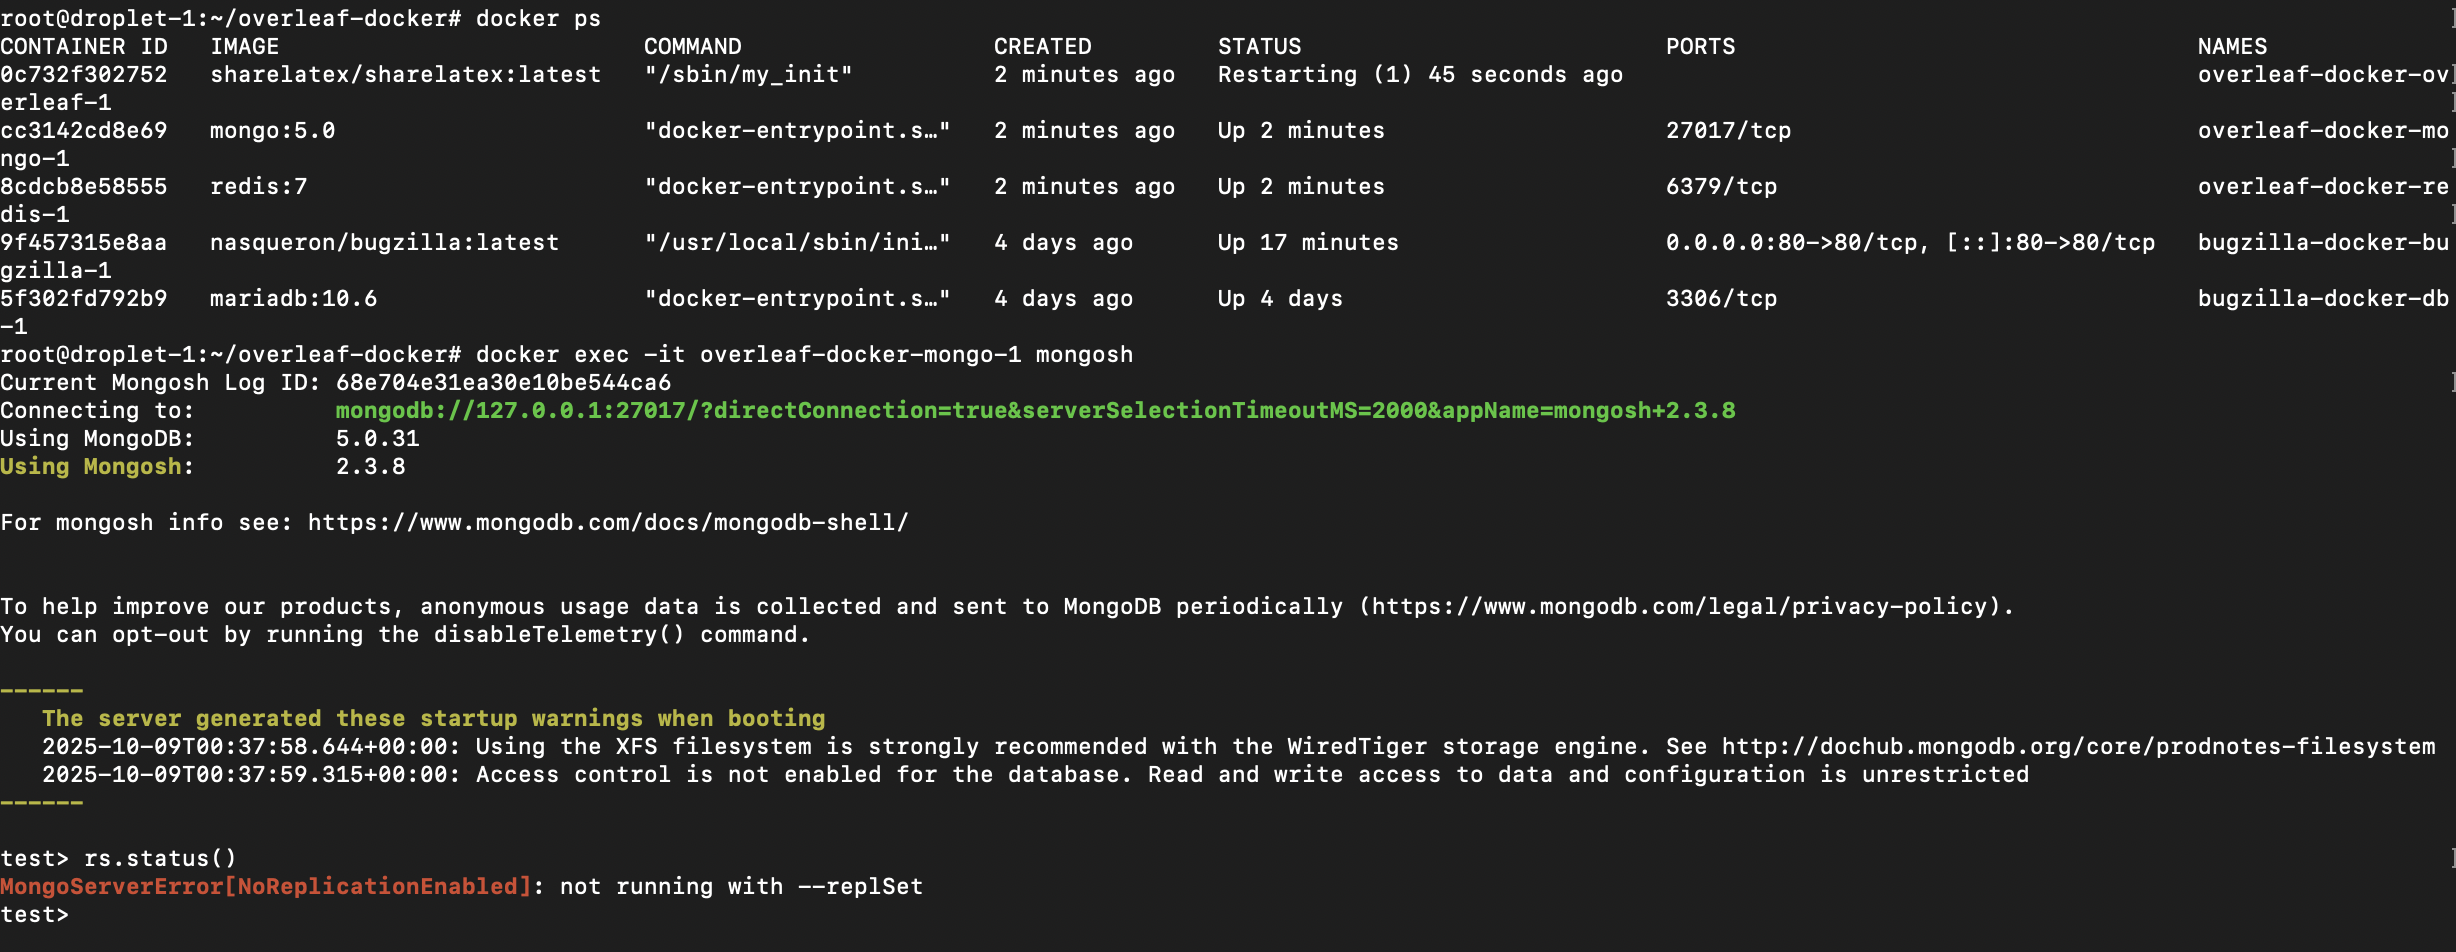
\includegraphics[width=1.0\linewidth]{png/restarting_problem_overleaf.png}
\end{figure}

This indicated that MongoDB was version 6.0, but its internal
\texttt{featureCompatibilityVersion (FCV)} was still set to 5.0.

\section{Fixing MongoDB Configuration}

\subsection{Step 1: Enter Mongo Shell}
\begin{minted}[fontsize=\small]{bash}
docker exec -it overleaf-docker-mongo-1 mongosh
\end{minted}

\subsection{Step 2: Initialize Replica Set}
\begin{minted}[fontsize=\small]{js}
rs.initiate()
\end{minted}

If you see \texttt{MongoServerError[AlreadyInitialized]}, it means it’s already set up — that’s fine.

\subsection{Step 3: Update Feature Compatibility Version}
\begin{minted}[fontsize=\small]{js}
use admin
db.adminCommand({ setFeatureCompatibilityVersion: "6.0" })
\end{minted}

Expected output:
\begin{minted}[fontsize=\small]{json}
{ "ok" : 1 }
\end{minted}

\subsection{Step 4: Restart Overleaf}
\begin{minted}[fontsize=\small]{bash}
exit
docker restart overleaf-docker-overleaf-1
\end{minted}


\section{Making Overleaf Publicly Accessible}

Since Bugzilla was already bound to port 80, Overleaf was assigned to port 8090.  
I confirmed the port was open:
\begin{minted}[fontsize=\small]{bash}
ss -tuln | grep 8090
\end{minted}

Then enabled it in the firewall:
\begin{minted}[fontsize=\small]{bash}
sudo ufw allow 8090/tcp
sudo ufw reload
\end{minted}

\section{Access and Verification}
Once restarted, Overleaf was reachable at:
\begin{minted}[fontsize=\small]{text}
http://174.138.68.199:8090
\end{minted}

I verified it via:
\begin{minted}[fontsize=\small]{bash}
curl -I http://174.138.68.199:8090
\end{minted}

Result:
\begin{minted}[fontsize=\small]{text}
HTTP/1.1 200 OK
\end{minted}

\section{Conclusion on Setting up Overleaf}
The deployment succeeded after:
\begin{enumerate}
  \item Gaining SSH access by adding my GitHub SSH key to the droplet.
  \item Running Overleaf on port 8090 (to avoid conflict with Bugzilla on port 80).
  \item Initializing the MongoDB replica set.
  \item Updating the MongoDB feature compatibility version to 6.0.
\end{enumerate}

After these steps, Overleaf was fully functional and accessible publicly via:
\begin{minted}[fontsize=\small]{text}
http://174.138.68.199:8090
\end{minted}

\begin{figure}
    \centering
    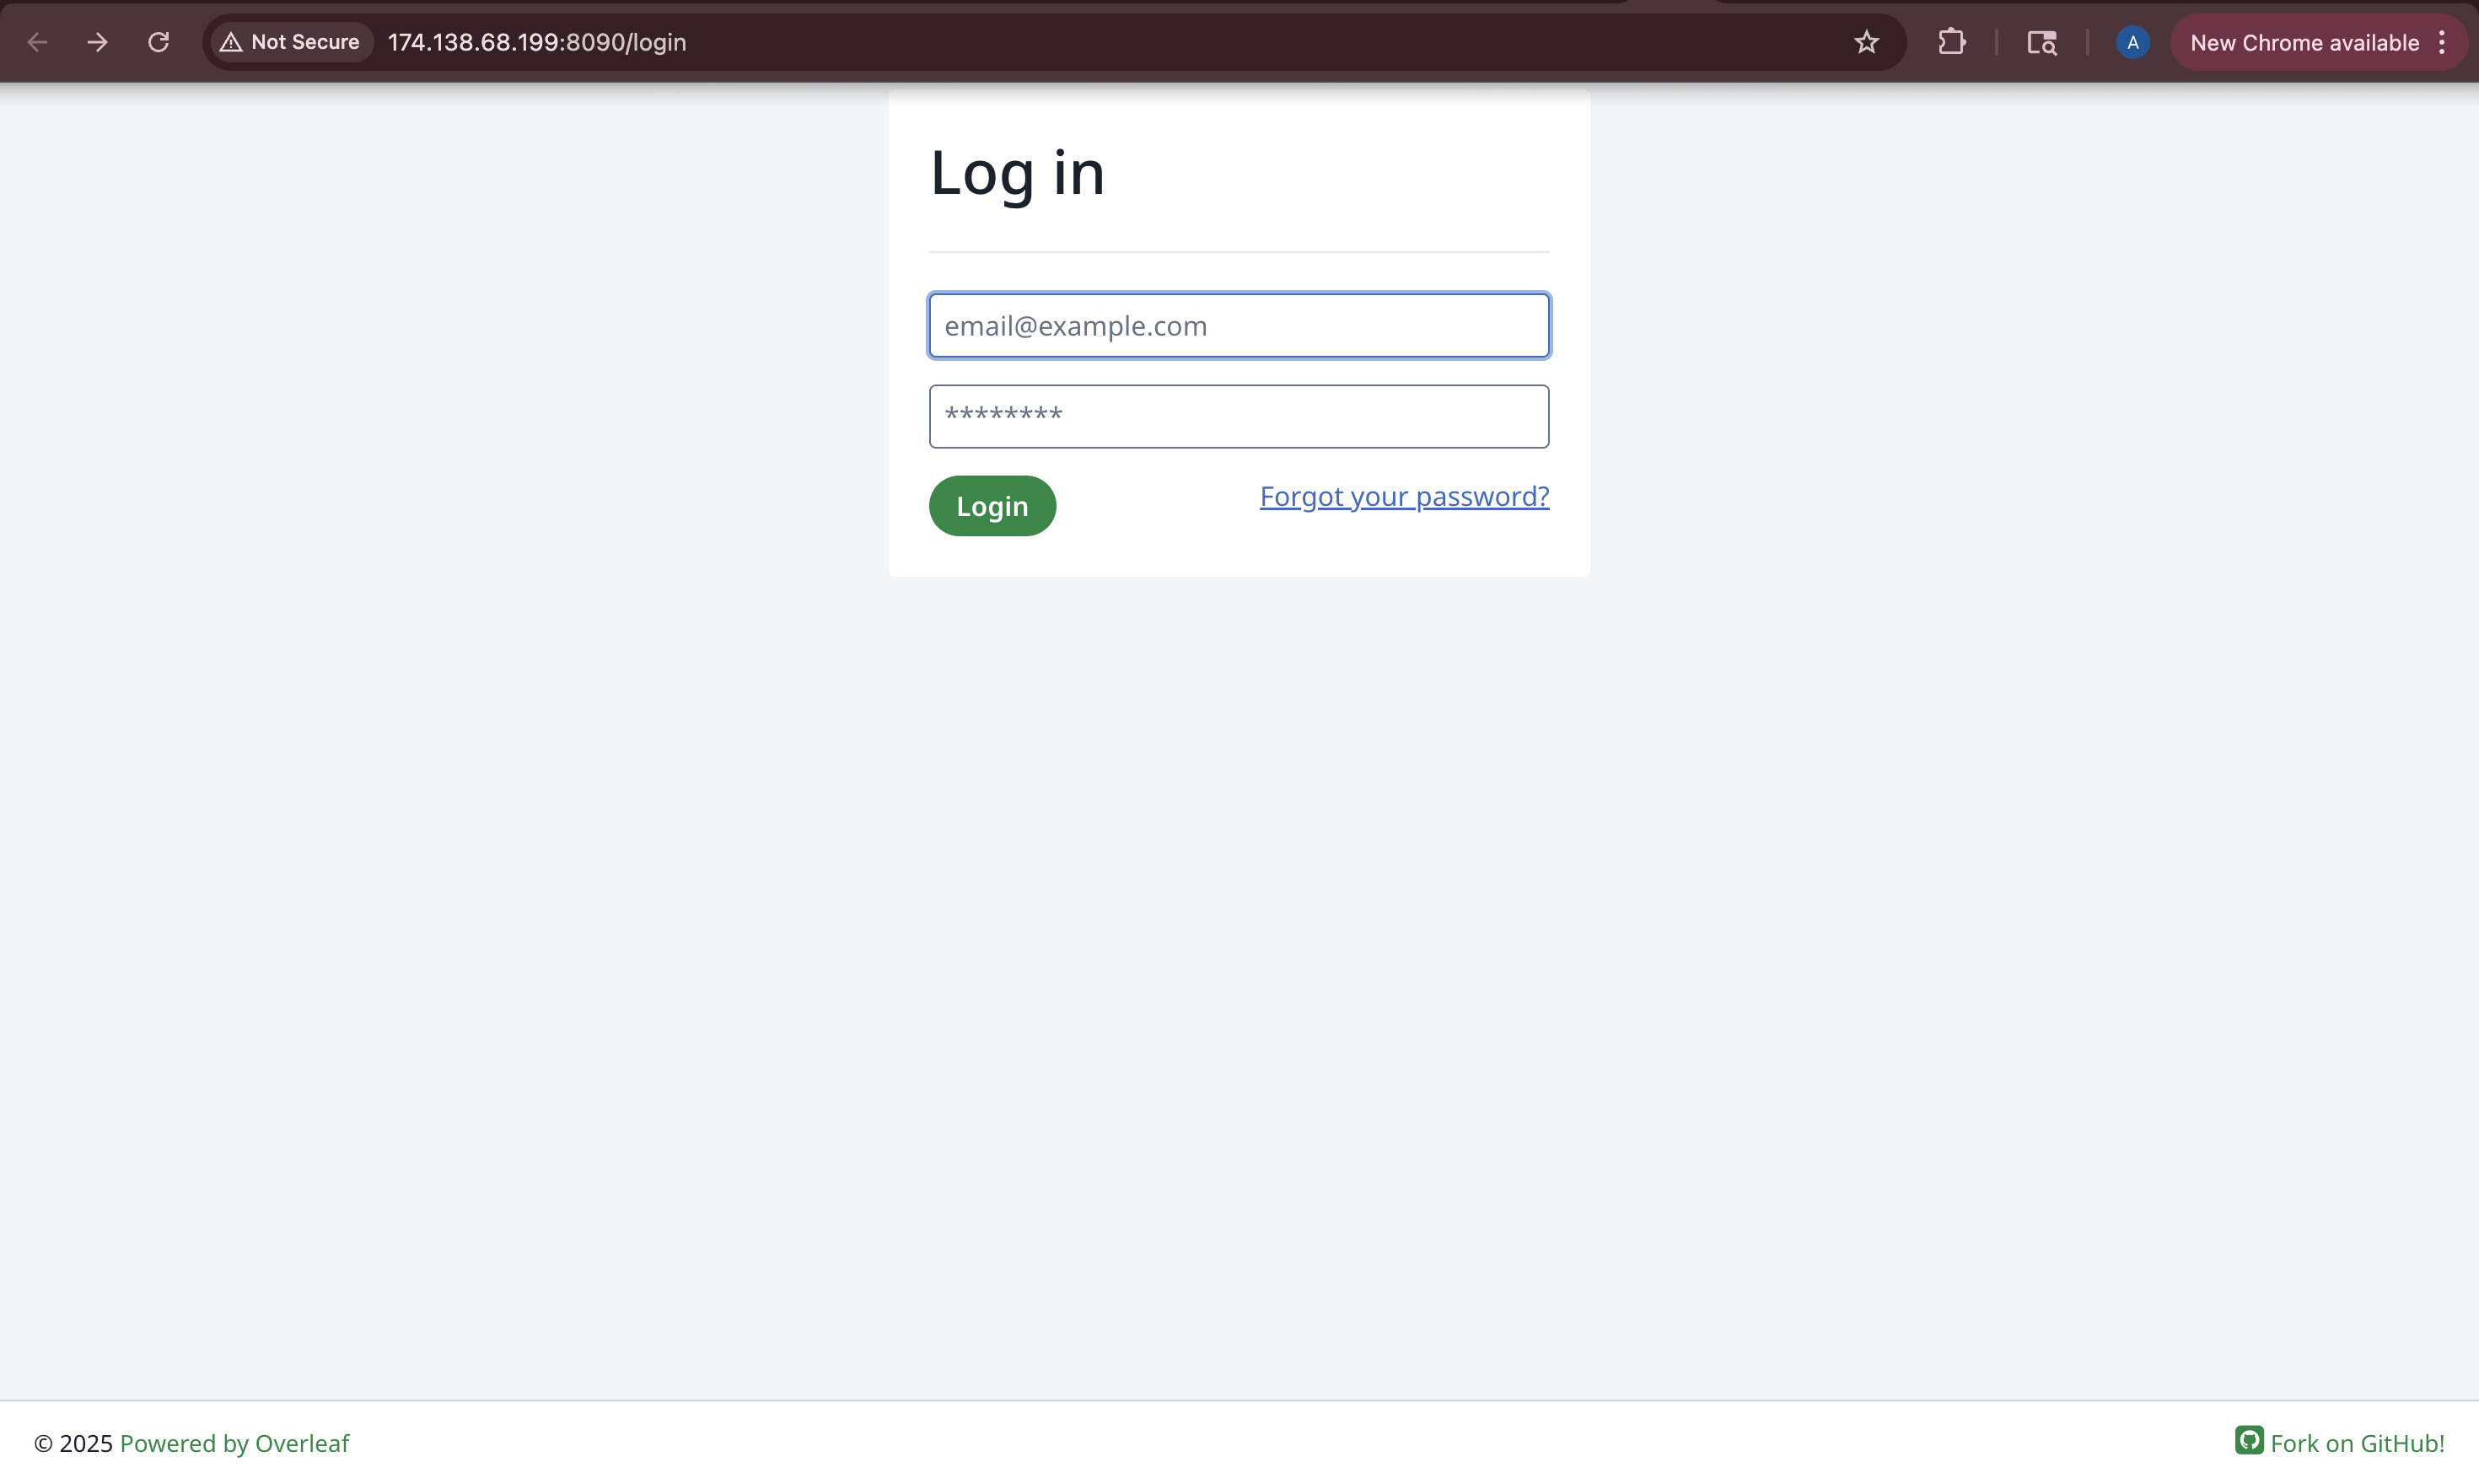
\includegraphics[width=1.0\linewidth]{png/overleaf running.png}
    \caption{overleaf website on http://174.138.68.199:8090}
    \label{fig:placeholder}
\end{figure}

This was what was seen:
\begin{figure}
    \centering
    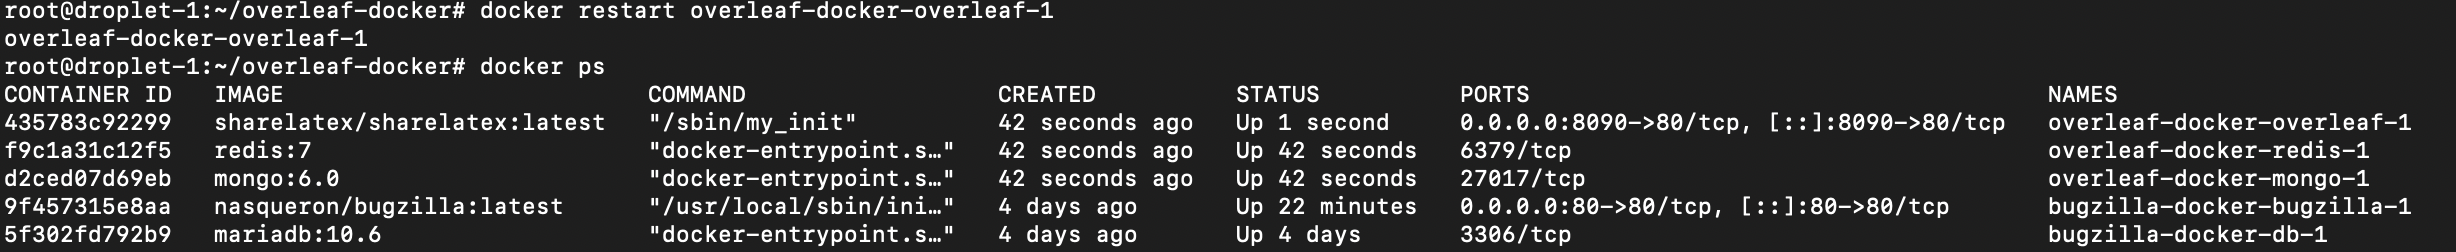
\includegraphics[width=1.0\linewidth]{png/finally_fixed.png}
\end{figure}

\section{Setting up Overleaf Packages}
Even thought Overleaf is up and running, we weren't able to run our document due to Overleaf not having access to any of the packages we were using. Thus we had to download the packages needed with commands:
\begin{minted}{bash}
apt-get update
apt-get install -y texlive-full
mktexlsr
\end{minted}
This took a long time to run, but afterwards our notebook was able to compile and had no errors in showing the pdf, however minted has refused to work even after installation... to fix the issue of packages corrupted or errors from minted I ran this command:
\begin{minted} {shell}
docker compose exec overleaf bash -lc '
  set -e
  export PATH=/usr/local/texlive/2025/bin/x86_64-linux:$PATH
  tlmgr option repository https://mirror.ctan.org/systems/texlive/tlnet
  tlmgr update --self
  tlmgr install scheme-full
  mktexlsr
'
\end{minted}
this command forced the packages to be correctly installed in the correct path.

\section{Domain Names, SSL}
Lets discuss the full process of deploying an Overleaf instance with a custom domain and secure HTTPS access on a DigitalOcean droplet.  

It includes:
\begin{itemize}
    \item Creating and mapping a custom subdomain (\texttt{overleaf-ssw590-team07.annanyajain.me}).
    \item Configuring \texttt{Nginx} as a reverse proxy for the Overleaf Docker container.
    \item Obtaining and applying a Let's Encrypt SSL certificate.
    \item Debugging HTTPS access until the setup functioned securely.
\end{itemize}

\section{Domain and Reverse Proxy Setup}
\subsection{DNS Configuration}
A subdomain was created in the DNS settings for \texttt{annanyajain.me} with the following record:
\begin{minted}{text}
Type: A
Host: overleaf-ssw590-team07
Value: 174.138.68.199
TTL: 3600
\end{minted}

We verified DNS propagation:
\begin{minted}{bash}
dig overleaf-ssw590-team07.annanyajain.me +short
174.138.68.199
\end{minted}

\subsection{Overleaf Docker Setup}
The Overleaf container was configured to listen on port \texttt{8090}:
\begin{minted}{bash}
sudo docker ps --format "table {{.Names}}\t{{.Ports}}"
overleaf-docker-overleaf-1   0.0.0.0:8090->80/tcp
\end{minted}

Verification:
\begin{minted}{bash}
curl -I http://localhost:8090/login
HTTP/1.1 302 Found
Location: /login
\end{minted}

\subsection{Nginx Reverse Proxy}
Nginx was used to route traffic from the public domain to the Overleaf container.  
Configuration file path:
\begin{minted}{bash}
/etc/nginx/sites-available/overleaf-https.conf
\end{minted}

File contents:
\begin{minted}{nginx}
server {
    listen 80;
    server_name overleaf-ssw590-team07.annanyajain.me;
    return 301 https://$host$request_uri;
}

server {
    listen 443 ssl;
    server_name overleaf-ssw590-team07.annanyajain.me;

    ssl_certificate /etc/letsencrypt/live/overleaf-ssw590-team07.annanyajain.me/fullchain.pem;
    ssl_certificate_key /etc/letsencrypt/live/overleaf-ssw590-team07.annanyajain.me/privkey.pem;

    ssl_protocols TLSv1.2 TLSv1.3;
    ssl_ciphers HIGH:!aNULL:!MD5;

    location / {
        proxy_pass http://localhost:8090;
        proxy_set_header Host $host;
        proxy_set_header X-Real-IP $remote_addr;
        proxy_set_header X-Forwarded-For $proxy_add_x_forwarded_for;
        proxy_set_header X-Forwarded-Proto $scheme;
    }
}
\end{minted}

Enabled and tested:
\begin{minted}{bash}
sudo ln -s /etc/nginx/sites-available/overleaf-https.conf /etc/nginx/sites-enabled/
sudo nginx -t
sudo systemctl restart nginx
\end{minted}

\section{SSL Certificates, Firewall, and Debugging}
\subsection{Firewall Configuration}
The firewall was configured to allow web and SSH access:
\begin{minted}{bash}
sudo ufw allow 80/tcp
sudo ufw allow 443/tcp
sudo ufw allow 8090/tcp
sudo ufw allow OpenSSH
sudo ufw enable
sudo ufw status
\end{minted}

\subsection{Obtaining an SSL Certificate}
Once HTTP (port 80) was accessible, a Let's Encrypt certificate was obtained:
\begin{minted}{bash}
sudo certbot certonly --nginx -d overleaf-ssw590-team07.annanyajain.me
\end{minted}

Certbot confirmed:
\begin{minted}{text}
Successfully received certificate.
Certificate is saved at:
/etc/letsencrypt/live/overleaf-ssw590-team07.annanyajain.me/fullchain.pem
Key is saved at:
/etc/letsencrypt/live/overleaf-ssw590-team07.annanyajain.me/privkey.pem
\end{minted}

\subsection{Verification}
Check certificate validity:
\begin{minted}{bash}
sudo openssl x509 -in /etc/letsencrypt/live/overleaf-ssw590-team07.annanyajain.me/fullchain.pem -noout -dates
notBefore=Oct 15 23:53:29 2025 GMT
notAfter=Jan 13 23:53:28 2026 GMT
\end{minted}

Confirm ports are open:
\begin{minted}{bash}
sudo ss -tuln | grep -E ':80|:443'
tcp LISTEN 0 511 0.0.0.0:443  0.0.0.0:*
tcp LISTEN 0 4096 0.0.0.0:80  0.0.0.0:*
\end{minted}

\subsection{Debugging HTTPS Access}
Initially, even with a valid Let's Encrypt certificate, HTTPS access failed.  
Local tests worked, but external connections hung during the TLS handshake:
\begin{minted}{bash}
curl -vk https://overleaf-ssw590-team07.annanyajain.me
# (Hangs during TLS handshake)
\end{minted}

\paragraph{Diagnosis:}
Nginx was confirmed to be listening:
\begin{minted}{bash}
sudo ss -tuln | grep :443
tcp LISTEN 0 511 0.0.0.0:443 0.0.0.0:*
\end{minted}
Thus, the issue was a blocked inbound port.

\paragraph{Fix:}
We explicitly reopened port 443:
\begin{minted}{bash}
sudo ufw allow 443/tcp
sudo ufw status
\end{minted}

\paragraph{Verification:}
After reopening the port, HTTPS immediately worked:
\begin{minted}{bash}
curl -vk https://overleaf-ssw590-team07.annanyajain.me
# SSL connection using TLSv1.3 / AEAD-AES256-GCM-SHA384
# SSL certificate verify ok.
# HTTP/1.1 302 Found -> /login
\end{minted}

External connection confirmed:
\begin{minted}{bash}
nc -vz overleaf-ssw590-team07.annanyajain.me 443
Connection to overleaf-ssw590-team07.annanyajain.me port 443 [tcp/https] succeeded!
\end{minted}

\subsection{Renewal}
Automatic renewal is managed by Certbot’s system timer.  
Manual renewal test:
\begin{minted}{bash}
sudo certbot renew --dry-run
\end{minted}

\subsection{Final Verification}
Overleaf is now securely available at:
\begin{itemize}
    \item \textbf{HTTPS (secure):} \href{https://overleaf-ssw590-team07.annanyajain.me}{https://overleaf-ssw590-team07.annanyajain.me}
    \item \textbf{HTTP (debug only):} \href{http://overleaf-ssw590-team07.annanyajain.me:81}{http://overleaf-ssw590-team07.annanyajain.me:81}
\end{itemize}

\noindent
\textbf{Results:}
\begin{itemize}
    \item Fully functional HTTPS via Let's Encrypt.
    \item Nginx reverse proxy routing traffic to Docker.
    \item Confirmed automatic certificate renewal.
    \item Firewall correctly configured and verified.
\end{itemize}

\section{Connecting Our Overleaf Instance to GitHub}
I first created a new empty GitHub Repository for Overleaf, and then connected to our droplet under where the Overleaf yaml file exists.

The workflow is as follows: \\
1. Overleaf CE is installed via Docker on a Droplet. \\
2. Overleaf project is connected to a GitHub repository (SSW590-team-7-Overleaf). \\
3. A GitHub Action builds the LaTeX document, adds version metadata, and commits the compiled PDF back to the repo automatically. \\

I first modified the Docker file:
\begin{minted}[fontsize=\small, bgcolor=gray!5, linenos]{yaml}
services:
  mongo:
    image: mongo:6.0
    restart: unless-stopped
    command: ["--replSet", "rs0", "--bind_ip_all"]
    volumes:
      - mongo_data:/data/db

  redis:
    image: redis:7
    restart: unless-stopped

  overleaf:
    image: sharelatex/sharelatex:latest
    restart: unless-stopped
    depends_on:
      - mongo
      - redis
    ports:
      - "8090:80"
    environment:
      - OVERLEAF_MONGO_URL=mongodb://mongo/sharelatex
      - OVERLEAF_REDIS_HOST=redis
      - OVERLEAF_MAX_UPLOAD_SIZE=50
      - V1_HISTORY_URL=http://overleaf:3100/api
    volumes:
      - ./data:/var/lib/overleaf

volumes:
  mongo_data:
\end{minted}

and then started the Overleaf again with the new file and checked if it was running correctly:
\begin{minted}{bash}
    docker compose up -d
    docker compose ps
\end{minted}

I created the new GitHub repo via their web interface, and then ran these commands to gain access and configure git identity:
\begin{minted}{bash}
    git clone git@github.com:cascadingluo/SSW590-team-7-Overleaf.git
    git config --global user.email "<email>"
git config --global user.name "<username>"
\end{minted}

I committed to initialize the project:
\begin{minted}{bash}
git add .
git commit -m "Initial LaTeX project"
git push -u origin main
\end{minted}

Then we created the workflow directory:
\begin{minted}{bash}
mkdir -p .github/workflows
\end{minted}
and then created the workflow file:
\begin{minted}[fontsize=\small, bgcolor=gray!5, linenos]{yaml}
name: Build PDF on push

on:
  push:
    branches: [ "main", "master" ]
  workflow_dispatch:
permissions:
  contents: write

jobs:
  build:
    runs-on: ubuntu-latest

    steps:
      - name: Checkout (full history)
        uses: actions/checkout@v4
        with:
          fetch-depth: 0

      - name: Create version.tex
        id: ver
        shell: bash
        run: |
          SHORT_SHA="$(git rev-parse --short HEAD)"
          CL_NUM="$(git rev-list --count HEAD)"
          RUN_NUM="${GITHUB_RUN_NUMBER}"
          DATE="$(date -u +'%Y-%m-%d')"
          {
            echo "short_sha=$SHORT_SHA"
            echo "cl_num=$CL_NUM"
            echo "run_num=$RUN_NUM"
            echo "date=$DATE"
          } >> "$GITHUB_OUTPUT"

          printf '%% Auto-generated by GitHub Actions\n' > version.tex
          printf '\\newcommand{\\builddate}{%s}\n' "$DATE" >> version.tex
          printf '\\newcommand{\\changeset}{%s}\n' "$SHORT_SHA" >> version.tex
          printf '\\newcommand{\\changelist}{%s}\n' "$CL_NUM" >> version.tex
          printf '\\newcommand{\\buildnum}{%s}\n' "$RUN_NUM" >> version.tex
          printf '%% Example: Version \\buildnum{} (CL \\changelist{}, SHA \\changeset{}, \\builddate{})\n' >> version.tex

      - name: Move version.tex next to itManual.tex
        run: |
          cp version.tex "2025F_SSW590_07-3/"

      - name: Build LaTeX
        uses: xu-cheng/latex-action@v3
        with:
          working_directory: "2025F_SSW590_07-3"
          root_file: itManual.tex
          latexmk_use_xelatex: true
          args: -norc -file-line-error -halt-on-error -interaction=nonstopmode -output-directory=. itManual.tex
          latexmk_shell_escape: true
         # pre_compile: |
           # cp ../version.tex .
           # apt-get update && apt-get install -y python3-pygments
          # Uncomment and edit if you need extra packages
          pre_compile: |
            echo "PATH=$PATH"
            tlmgr option repository https://mirror.ctan.org/systems/texlive/tlnet
            tlmgr update --self
            tlmgr install minted fvextra fancyvrb framed upquote lineno xcolor etoolbox siunitx titlesec caption pgfplots

      - name: Save and commit PDF
        run: |
          mkdir -p builds

      - name: Save and commit PDF
        run: |
          cp "2025F_SSW590_07-3/itManual.pdf" "builds/itManual_${{ github.sha }}.pdf"

      - name: Upload PDF
        uses: actions/upload-artifact@v4
        with:
          name: itManual
          path: builds/itManual_${{ github. sha}}.pdf

      - name: Set GitHub user config
        run: |
          git config user.name  "github-actions[bot]"
          git config user.email "github-actions[bot]@users.noreply.github.com"
          git add builds/*.pdf version.tex
          git commit -m "CI: build PDF CL=${{ steps.ver.outputs.changelist }}" || exit 0
          git push

      - name: Clean LaTeX build files
        run: |
          rm -f *.aux *.log *.out *.toc *.fdb_latexmk *.fls
\end{minted}

After creating this file we linked it with overleaf and allowed it to auto create a new version every time we pushed into github. 

In order to add versioning, we went into the itManual.tex file and added:
\begin{minted}{bash}
input{version.tex}
\end{minted}

This allowed us to use the github variables inside the LaTeX document which we used in:

\begin{minted}{bash}
Version buildnum{} Cl changelist{} SHA changeset{} and builddate{}
\end{minted}

I tested the workflow by triggering the action:
\begin{minted}{bash}
git add .
git commit -m "Test Overleaf GitHub build"
git pull --rebase origin main
git push
\end{minted}

We created a file for syncing github with our server overleaf:
\begin{minted} {bash}
#!/bin/bash
# === Configuration ===
CONTAINER_NAME="overleaf-docker-overleaf-1"
PROJECT_PATH="/var/lib/overleaf/data/compiles/68eabaec5adfde60821a1298-68eab97f534beb493f28d48a"
GITHUB_REPO_PATH="/root/overleaf-docker/ssw590-overleaf"
TARGET_SUBFOLDER="2025F_SSW590_07-3"

# === Sync Overleaf project into GitHub repo ===
echo "Copying project from container to GitHub repo..."
docker cp "${CONTAINER_NAME}:${PROJECT_PATH}/." "${GITHUB_REPO_PATH}/${TARGET_SUBFOLDER}/"

cd "$GITHUB_REPO_PATH" || exit

# === Commit and push ===
git add .
git commit -m "Auto-sync from Overleaf container on $(date -u +'%Y-%m-%d %H:%M:%S')" || true
git push origin main
\end{minted}

Whenever we update the files on our Overleaf, we run:
\begin{minted} {bash}
./sync_overleaf_to_github.sh
\end{minted}
to sync all of our changes.

\\

